% Options for packages loaded elsewhere
\PassOptionsToPackage{unicode}{hyperref}
\PassOptionsToPackage{hyphens}{url}
%
\documentclass[
]{article}
\usepackage{amsmath,amssymb}
\usepackage{iftex}
\ifPDFTeX
  \usepackage[T1]{fontenc}
  \usepackage[utf8]{inputenc}
  \usepackage{textcomp} % provide euro and other symbols
\else % if luatex or xetex
  \usepackage{unicode-math} % this also loads fontspec
  \defaultfontfeatures{Scale=MatchLowercase}
  \defaultfontfeatures[\rmfamily]{Ligatures=TeX,Scale=1}
\fi
\usepackage{lmodern}
\ifPDFTeX\else
  % xetex/luatex font selection
\fi
% Use upquote if available, for straight quotes in verbatim environments
\IfFileExists{upquote.sty}{\usepackage{upquote}}{}
\IfFileExists{microtype.sty}{% use microtype if available
  \usepackage[]{microtype}
  \UseMicrotypeSet[protrusion]{basicmath} % disable protrusion for tt fonts
}{}
\makeatletter
\@ifundefined{KOMAClassName}{% if non-KOMA class
  \IfFileExists{parskip.sty}{%
    \usepackage{parskip}
  }{% else
    \setlength{\parindent}{0pt}
    \setlength{\parskip}{6pt plus 2pt minus 1pt}}
}{% if KOMA class
  \KOMAoptions{parskip=half}}
\makeatother
\usepackage{xcolor}
\usepackage[margin=1in]{geometry}
\usepackage{color}
\usepackage{fancyvrb}
\newcommand{\VerbBar}{|}
\newcommand{\VERB}{\Verb[commandchars=\\\{\}]}
\DefineVerbatimEnvironment{Highlighting}{Verbatim}{commandchars=\\\{\}}
% Add ',fontsize=\small' for more characters per line
\usepackage{framed}
\definecolor{shadecolor}{RGB}{248,248,248}
\newenvironment{Shaded}{\begin{snugshade}}{\end{snugshade}}
\newcommand{\AlertTok}[1]{\textcolor[rgb]{0.94,0.16,0.16}{#1}}
\newcommand{\AnnotationTok}[1]{\textcolor[rgb]{0.56,0.35,0.01}{\textbf{\textit{#1}}}}
\newcommand{\AttributeTok}[1]{\textcolor[rgb]{0.13,0.29,0.53}{#1}}
\newcommand{\BaseNTok}[1]{\textcolor[rgb]{0.00,0.00,0.81}{#1}}
\newcommand{\BuiltInTok}[1]{#1}
\newcommand{\CharTok}[1]{\textcolor[rgb]{0.31,0.60,0.02}{#1}}
\newcommand{\CommentTok}[1]{\textcolor[rgb]{0.56,0.35,0.01}{\textit{#1}}}
\newcommand{\CommentVarTok}[1]{\textcolor[rgb]{0.56,0.35,0.01}{\textbf{\textit{#1}}}}
\newcommand{\ConstantTok}[1]{\textcolor[rgb]{0.56,0.35,0.01}{#1}}
\newcommand{\ControlFlowTok}[1]{\textcolor[rgb]{0.13,0.29,0.53}{\textbf{#1}}}
\newcommand{\DataTypeTok}[1]{\textcolor[rgb]{0.13,0.29,0.53}{#1}}
\newcommand{\DecValTok}[1]{\textcolor[rgb]{0.00,0.00,0.81}{#1}}
\newcommand{\DocumentationTok}[1]{\textcolor[rgb]{0.56,0.35,0.01}{\textbf{\textit{#1}}}}
\newcommand{\ErrorTok}[1]{\textcolor[rgb]{0.64,0.00,0.00}{\textbf{#1}}}
\newcommand{\ExtensionTok}[1]{#1}
\newcommand{\FloatTok}[1]{\textcolor[rgb]{0.00,0.00,0.81}{#1}}
\newcommand{\FunctionTok}[1]{\textcolor[rgb]{0.13,0.29,0.53}{\textbf{#1}}}
\newcommand{\ImportTok}[1]{#1}
\newcommand{\InformationTok}[1]{\textcolor[rgb]{0.56,0.35,0.01}{\textbf{\textit{#1}}}}
\newcommand{\KeywordTok}[1]{\textcolor[rgb]{0.13,0.29,0.53}{\textbf{#1}}}
\newcommand{\NormalTok}[1]{#1}
\newcommand{\OperatorTok}[1]{\textcolor[rgb]{0.81,0.36,0.00}{\textbf{#1}}}
\newcommand{\OtherTok}[1]{\textcolor[rgb]{0.56,0.35,0.01}{#1}}
\newcommand{\PreprocessorTok}[1]{\textcolor[rgb]{0.56,0.35,0.01}{\textit{#1}}}
\newcommand{\RegionMarkerTok}[1]{#1}
\newcommand{\SpecialCharTok}[1]{\textcolor[rgb]{0.81,0.36,0.00}{\textbf{#1}}}
\newcommand{\SpecialStringTok}[1]{\textcolor[rgb]{0.31,0.60,0.02}{#1}}
\newcommand{\StringTok}[1]{\textcolor[rgb]{0.31,0.60,0.02}{#1}}
\newcommand{\VariableTok}[1]{\textcolor[rgb]{0.00,0.00,0.00}{#1}}
\newcommand{\VerbatimStringTok}[1]{\textcolor[rgb]{0.31,0.60,0.02}{#1}}
\newcommand{\WarningTok}[1]{\textcolor[rgb]{0.56,0.35,0.01}{\textbf{\textit{#1}}}}
\usepackage{longtable,booktabs,array}
\usepackage{calc} % for calculating minipage widths
% Correct order of tables after \paragraph or \subparagraph
\usepackage{etoolbox}
\makeatletter
\patchcmd\longtable{\par}{\if@noskipsec\mbox{}\fi\par}{}{}
\makeatother
% Allow footnotes in longtable head/foot
\IfFileExists{footnotehyper.sty}{\usepackage{footnotehyper}}{\usepackage{footnote}}
\makesavenoteenv{longtable}
\usepackage{graphicx}
\makeatletter
\def\maxwidth{\ifdim\Gin@nat@width>\linewidth\linewidth\else\Gin@nat@width\fi}
\def\maxheight{\ifdim\Gin@nat@height>\textheight\textheight\else\Gin@nat@height\fi}
\makeatother
% Scale images if necessary, so that they will not overflow the page
% margins by default, and it is still possible to overwrite the defaults
% using explicit options in \includegraphics[width, height, ...]{}
\setkeys{Gin}{width=\maxwidth,height=\maxheight,keepaspectratio}
% Set default figure placement to htbp
\makeatletter
\def\fps@figure{htbp}
\makeatother
\setlength{\emergencystretch}{3em} % prevent overfull lines
\providecommand{\tightlist}{%
  \setlength{\itemsep}{0pt}\setlength{\parskip}{0pt}}
\setcounter{secnumdepth}{-\maxdimen} % remove section numbering
\ifLuaTeX
  \usepackage{selnolig}  % disable illegal ligatures
\fi
\IfFileExists{bookmark.sty}{\usepackage{bookmark}}{\usepackage{hyperref}}
\IfFileExists{xurl.sty}{\usepackage{xurl}}{} % add URL line breaks if available
\urlstyle{same}
\hypersetup{
  pdftitle={checkin\_feb\_20\_deliverable},
  pdfauthor={Allison Stewart, Christine Kuryla, Zander De Jesus, Alana Ferris},
  hidelinks,
  pdfcreator={LaTeX via pandoc}}

\title{checkin\_feb\_20\_deliverable}
\author{Allison Stewart, Christine Kuryla, Zander De Jesus, Alana
Ferris}
\date{2024-02-19}

\begin{document}
\maketitle

\hypertarget{research-question}{%
\section{Research Question}\label{research-question}}

Does exposure to phthalate alternatives affect inflammation in children
as measured by alpha-1-acid glycoprotein? We will investigate this
question using NHANES data from 2017-2018 of the serum inflammatory
biomarker alpha-1-acid glycoprotein and urinary phthalate alternative
metabolite levels, along with other relevant data (urinary creatinine
levels and sociodemographic data).

\hypertarget{reading-in-relevant-nhanes-2017-2018-data}{%
\section{reading in relevant NHANES 2017-2018
data}\label{reading-in-relevant-nhanes-2017-2018-data}}

\begin{itemize}
\tightlist
\item
  NOTE: phthalate and AGP data have special sample weights we need to
  account for in analysis
\item
  weighting module:
  \url{https://wwwn.cdc.gov/nchs/nhanes/tutorials/Weighting.aspx}
\end{itemize}

\begin{Shaded}
\begin{Highlighting}[]
\CommentTok{\# phthalates and plasticizers metabolites {-} urine }
\CommentTok{\# codebook, LODs: https://wwwn.cdc.gov/Nchs/Nhanes/2017{-}2018/PHTHTE\_J.htm}
\NormalTok{phthte\_urine }\OtherTok{=}
  \FunctionTok{read.xport}\NormalTok{(}\StringTok{"data/PHTHTE\_J.XPT"}\NormalTok{) }\SpecialCharTok{\%\textgreater{}\%} 
\NormalTok{  janitor}\SpecialCharTok{::}\FunctionTok{clean\_names}\NormalTok{()}

\CommentTok{\# urine creatinine levels }
\CommentTok{\# codebook: https://wwwn.cdc.gov/Nchs/Nhanes/2017{-}2018/ALB\_CR\_J.htm}
\NormalTok{creatinine\_urine }\OtherTok{=}
  \FunctionTok{read.xport}\NormalTok{(}\StringTok{"data/ALB\_CR\_J.XPT"}\NormalTok{) }\SpecialCharTok{\%\textgreater{}\%} 
\NormalTok{  janitor}\SpecialCharTok{::}\FunctionTok{clean\_names}\NormalTok{()}

\CommentTok{\# Alpha{-}1{-}Acid Glycoprotein {-} Serum}
\CommentTok{\# codebook: https://wwwn.cdc.gov/Nchs/Nhanes/2017{-}2018/SSAGP\_J.htm}
\NormalTok{agp\_serum }\OtherTok{=}
  \FunctionTok{read.xport}\NormalTok{(}\StringTok{"data/SSAGP\_J.XPT"}\NormalTok{) }\SpecialCharTok{\%\textgreater{}\%} 
\NormalTok{  janitor}\SpecialCharTok{::}\FunctionTok{clean\_names}\NormalTok{()}

\CommentTok{\# Demographic variables and sample weights }
\CommentTok{\# codebook: https://wwwn.cdc.gov/Nchs/Nhanes/2017{-}2018/DEMO\_J.htm}
\NormalTok{demo }\OtherTok{=}
  \FunctionTok{read.xport}\NormalTok{(}\StringTok{"data/DEMO\_J.XPT"}\NormalTok{) }\SpecialCharTok{|\textgreater{}} 
\NormalTok{  janitor}\SpecialCharTok{::}\FunctionTok{clean\_names}\NormalTok{()}
\end{Highlighting}
\end{Shaded}

\hypertarget{cleaning-variable-names-of-phthalate-urine-data}{%
\section{cleaning variable names of phthalate urine
data}\label{cleaning-variable-names-of-phthalate-urine-data}}

\begin{Shaded}
\begin{Highlighting}[]
\NormalTok{phthte\_urine }\OtherTok{=}
\NormalTok{  phthte\_urine }\SpecialCharTok{\%\textgreater{}\%} 
  \FunctionTok{rename}\NormalTok{(}\AttributeTok{weights =}\NormalTok{ wtsb2yr) }\SpecialCharTok{\%\textgreater{}\%}
  \FunctionTok{rename\_with}\NormalTok{(}\SpecialCharTok{\textasciitilde{}} \FunctionTok{gsub}\NormalTok{(}\StringTok{"\^{}urx"}\NormalTok{, }\StringTok{""}\NormalTok{, .), }\FunctionTok{starts\_with}\NormalTok{(}\StringTok{"urx"}\NormalTok{))}
  
\CommentTok{\# for now, leaving the \textless{}LOD comment columns (i.e, columns started wit urd) as they are }
\CommentTok{\# 2986 obs}
\end{Highlighting}
\end{Shaded}

\hypertarget{merging-phthalate-urine-data-with-urinary-creatinine-levels-and-then-adjusting-concentrations-for-creatinine}{%
\section{merging phthalate urine data with urinary creatinine levels and
then adjusting concentrations for
creatinine}\label{merging-phthalate-urine-data-with-urinary-creatinine-levels-and-then-adjusting-concentrations-for-creatinine}}

\begin{Shaded}
\begin{Highlighting}[]
\CommentTok{\# dropping albumin from creatinine dataset}
\NormalTok{creatinine\_urine }\OtherTok{=}
\NormalTok{  creatinine\_urine }\SpecialCharTok{\%\textgreater{}\%} 
  \FunctionTok{select}\NormalTok{(seqn, urxucr, urducrlc) }\CommentTok{\#dropping urxcrs bc i dont want creatinine expressed in those units}
\CommentTok{\#7936 obs}

\CommentTok{\#merging creatinine data with phthalate data}
\NormalTok{phthte\_creatinine }\OtherTok{=}
  \FunctionTok{merge}\NormalTok{(creatinine\_urine, phthte\_urine, }\AttributeTok{by =} \StringTok{"seqn"}\NormalTok{) }\SpecialCharTok{\%\textgreater{}\%}
  \FunctionTok{select}\NormalTok{(}\SpecialCharTok{!}\FunctionTok{starts\_with}\NormalTok{(}\StringTok{"urd"}\NormalTok{)) }\SpecialCharTok{\%\textgreater{}\%} \CommentTok{\#dropped \textless{}LOD columns for ease of pivoting}
  \FunctionTok{pivot\_longer}\NormalTok{(}\AttributeTok{cols =}\NormalTok{ cnp}\SpecialCharTok{:}\NormalTok{mzp,  }
               \AttributeTok{names\_to =} \StringTok{"analyte\_code"}\NormalTok{,}
               \AttributeTok{values\_to =} \StringTok{"reported\_result"}\NormalTok{) }\CommentTok{\#pivoted longer so that i can map in the next step}

\CommentTok{\#56734 obs }

\CommentTok{\#urinary [phth] in ng/mL}
\CommentTok{\# urinary [creatinine] in mg/dL so need to get this to ng/mL}

\CommentTok{\# Urinary creatinine concentrations, specific gravity, and osmolality are common methods for adjusting dilution. The most widely used method is creatinine adjustment that involves dividing the analyte concentration by the creatinine concentration. Analyte results are then reported as weight of analyte per gram of creatinine (micrograms analyte per gram creatinine).}

\CommentTok{\# making a new column with creatinine{-}adjusted [phthalate]}
\NormalTok{phthte\_creatinine }\OtherTok{=}
\NormalTok{  phthte\_creatinine }\SpecialCharTok{\%\textgreater{}\%} 
  \FunctionTok{mutate}\NormalTok{(}\AttributeTok{ng\_per\_ml\_creatinine =}\NormalTok{ urxucr}\SpecialCharTok{*}\DecValTok{10000}\NormalTok{) }\SpecialCharTok{\%\textgreater{}\%} \CommentTok{\#here converting mg/dL to ng/mL{-}{-}\textgreater{} 1mg/dL = 10,000ng/mL}
  \FunctionTok{mutate}\NormalTok{(}\AttributeTok{adj\_conc =}\NormalTok{ reported\_result}\SpecialCharTok{/}\NormalTok{ng\_per\_ml\_creatinine)}

\CommentTok{\#visualizing adjusted concentrations but on the log scale bc the numbers are now so small lol ... i wonder if im just being dumb or if NHANES really doesnt report specific gravity data }
\FunctionTok{boxplot}\NormalTok{(}\FunctionTok{log10}\NormalTok{(phthte\_creatinine}\SpecialCharTok{$}\NormalTok{adj\_conc))}
\end{Highlighting}
\end{Shaded}

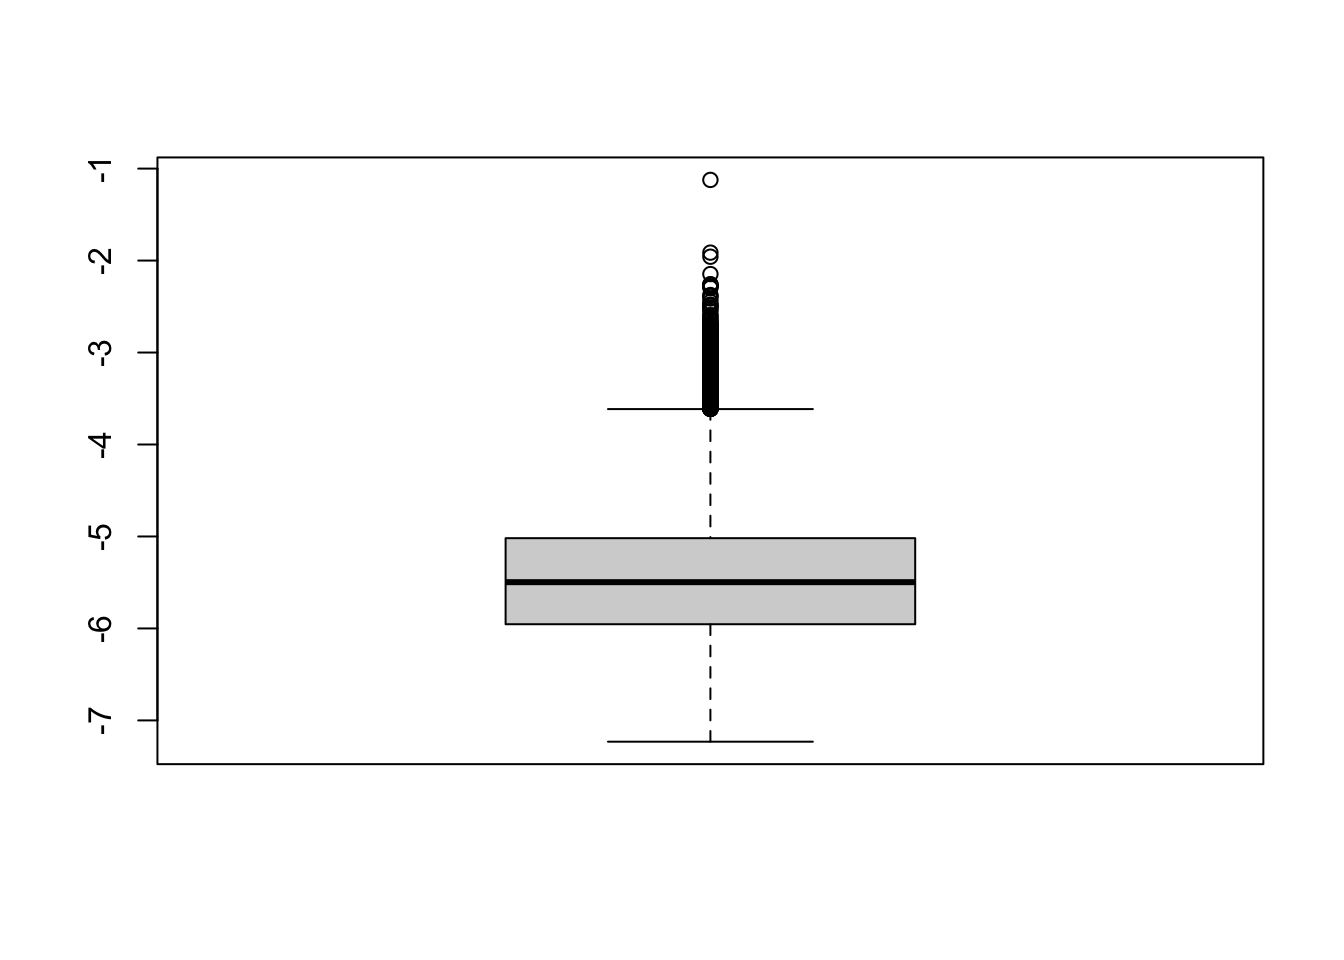
\includegraphics{checkin_feb_20_deliverable_files/figure-latex/unnamed-chunk-3-1.pdf}

\begin{Shaded}
\begin{Highlighting}[]
\FunctionTok{hist}\NormalTok{(}\FunctionTok{log10}\NormalTok{(phthte\_creatinine}\SpecialCharTok{$}\NormalTok{adj\_conc))}
\end{Highlighting}
\end{Shaded}

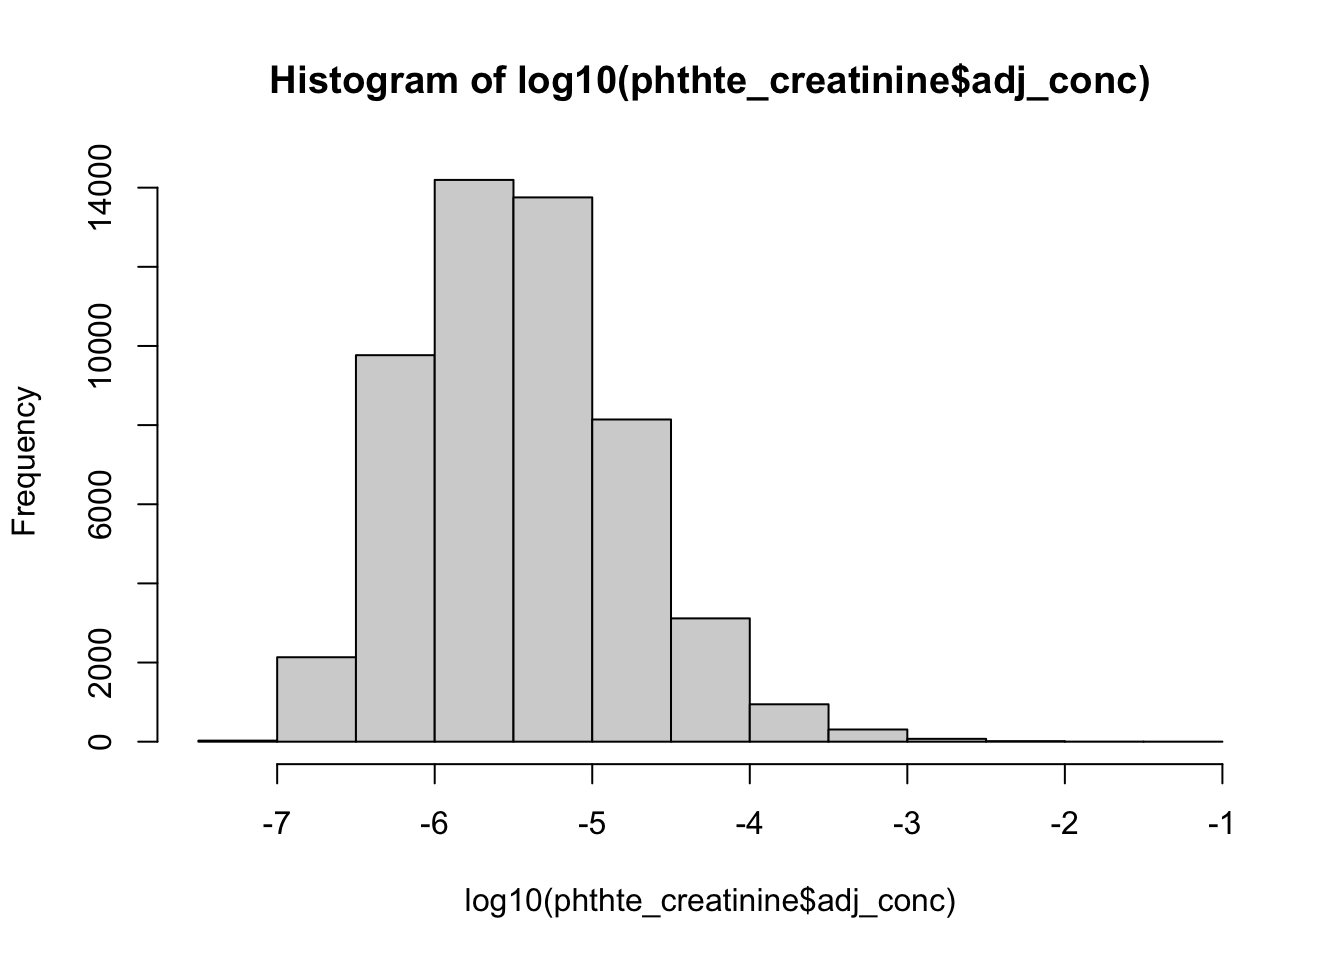
\includegraphics{checkin_feb_20_deliverable_files/figure-latex/unnamed-chunk-3-2.pdf}

\begin{Shaded}
\begin{Highlighting}[]
\DocumentationTok{\#\#\#dont log transform here\#\#\#}
\end{Highlighting}
\end{Shaded}

\hypertarget{cleaning-variables-name-of-demographic-data-and-drop-unneeded-variables}{%
\section{cleaning variables name of demographic data and drop unneeded
variables}\label{cleaning-variables-name-of-demographic-data-and-drop-unneeded-variables}}

\begin{Shaded}
\begin{Highlighting}[]
\NormalTok{demo }\OtherTok{\textless{}{-}} \FunctionTok{subset}\NormalTok{(demo, }\AttributeTok{select =} \SpecialCharTok{{-}}\FunctionTok{c}\NormalTok{(sddsrvyr, ridstatr, ridexprg, dmdmartl, dmdeduc2, dmqmiliz, dmqadfc, dmdhrgnd, dmdhragz, dmdhredz, dmdhrmaz, dmdhsedz))}

\NormalTok{demo }\OtherTok{\textless{}{-}}\NormalTok{ demo }\SpecialCharTok{|\textgreater{}} 
  \FunctionTok{rename}\NormalTok{(}\AttributeTok{gender =}\NormalTok{ riagendr, }
         \AttributeTok{age\_yrs\_screen =}\NormalTok{ ridageyr, }
         \AttributeTok{age\_mon\_screen =}\NormalTok{ ridagemn, }
         \AttributeTok{race\_ethn1 =}\NormalTok{ ridreth1,}
         \AttributeTok{race\_ethn3 =}\NormalTok{ ridreth3, }
         \AttributeTok{time\_period =}\NormalTok{ ridexmon, }
         \AttributeTok{age\_mon\_screen =}\NormalTok{ ridagemn,}
         \AttributeTok{age\_mon\_exam =}\NormalTok{ ridexagm, }
         \AttributeTok{birth\_country =}\NormalTok{ dmdborn4, }
         \AttributeTok{citizenship =}\NormalTok{ dmdcitzn,}
         \AttributeTok{years\_us =}\NormalTok{ dmdyrsus, }
         \AttributeTok{education =}\NormalTok{ dmdeduc3, }
         \AttributeTok{lang\_pers\_quest =}\NormalTok{ sialang, }
         \AttributeTok{proxy\_pers\_quest =}\NormalTok{ siaproxy, }
         \AttributeTok{interpret\_pers\_quest =}\NormalTok{ siaintrp, }
         \AttributeTok{lang\_fam\_interview =}\NormalTok{ fialang, }
         \AttributeTok{proxy\_fam\_interview =}\NormalTok{ fiaproxy, }
         \AttributeTok{interpret\_fam\_interview =}\NormalTok{ fiaintrp,}
         \AttributeTok{lang\_capi =}\NormalTok{ mialang, }
         \AttributeTok{proxy\_capi =}\NormalTok{ miaproxy, }
         \AttributeTok{interpret\_capi =}\NormalTok{ miaintrp, }
         \AttributeTok{lang\_acasi =}\NormalTok{ aialanga, }
         \AttributeTok{hh\_size =}\NormalTok{ dmdhhsiz, }
         \AttributeTok{fam\_size =}\NormalTok{ dmdfmsiz, }
         \AttributeTok{hh\_young\_children =}\NormalTok{ dmdhhsza,}
         \AttributeTok{hh\_children =}\NormalTok{ dmdhhszb, }
         \AttributeTok{hh\_adults =}\NormalTok{ dmdhhsze, }
         \AttributeTok{weight\_2yr\_intervew =}\NormalTok{ wtint2yr,}
         \AttributeTok{weight\_2yr\_mec =}\NormalTok{ wtmec2yr, }
         \AttributeTok{variance\_psu =}\NormalTok{ sdmvpsu, }
         \AttributeTok{variance\_stratum =}\NormalTok{ sdmvstra, }
         \AttributeTok{income\_hh\_annual =}\NormalTok{ indhhin2, }
         \AttributeTok{income\_family\_annual =}\NormalTok{ indfmin2, }
         \AttributeTok{income\_poverty\_ratio =}\NormalTok{ indfmpir)}
\end{Highlighting}
\end{Shaded}

\hypertarget{subset-to-ages-3-16}{%
\section{subset to ages 3-16}\label{subset-to-ages-3-16}}

\begin{Shaded}
\begin{Highlighting}[]
\NormalTok{demo }\OtherTok{\textless{}{-}}\NormalTok{ demo }\SpecialCharTok{|\textgreater{}} 
  \FunctionTok{filter}\NormalTok{(age\_yrs\_screen }\SpecialCharTok{\textgreater{}=} \DecValTok{3} \SpecialCharTok{\&}\NormalTok{ age\_yrs\_screen }\SpecialCharTok{\textless{}=} \DecValTok{16}\NormalTok{)}
\end{Highlighting}
\end{Shaded}

\hypertarget{create-table-1-with-age-gender-raceethnicity-and-household-income}{%
\section{create table 1 with age, gender, race/ethnicity, and household
income}\label{create-table-1-with-age-gender-raceethnicity-and-household-income}}

\begin{Shaded}
\begin{Highlighting}[]
\CommentTok{\# recode age into age group }
\NormalTok{demo }\OtherTok{\textless{}{-}}\NormalTok{ demo }\SpecialCharTok{|\textgreater{}} 
  \FunctionTok{mutate}\NormalTok{(}\AttributeTok{age\_group =} \FunctionTok{case\_when}\NormalTok{(age\_yrs\_screen }\SpecialCharTok{\textgreater{}=} \DecValTok{3} \SpecialCharTok{\&}\NormalTok{ age\_yrs\_screen }\SpecialCharTok{\textless{}} \DecValTok{7} \SpecialCharTok{\textasciitilde{}} \DecValTok{1}\NormalTok{,}
\NormalTok{                                          age\_yrs\_screen }\SpecialCharTok{\textgreater{}=} \DecValTok{7} \SpecialCharTok{\&}\NormalTok{ age\_yrs\_screen }\SpecialCharTok{\textless{}} \DecValTok{11} \SpecialCharTok{\textasciitilde{}} \DecValTok{2}\NormalTok{, }
\NormalTok{                                          age\_yrs\_screen }\SpecialCharTok{\textgreater{}=} \DecValTok{11} \SpecialCharTok{\&}\NormalTok{ age\_yrs\_screen }\SpecialCharTok{\textless{}} \DecValTok{14} \SpecialCharTok{\textasciitilde{}} \DecValTok{3}\NormalTok{, }
\NormalTok{                                          age\_yrs\_screen }\SpecialCharTok{\textgreater{}=} \DecValTok{14} \SpecialCharTok{\textasciitilde{}} \DecValTok{4}\NormalTok{,}
                                          \ConstantTok{TRUE} \SpecialCharTok{\textasciitilde{}} \ConstantTok{NA\_real\_}\NormalTok{))}

\CommentTok{\# recode household income into fewer categories }
\NormalTok{demo }\OtherTok{\textless{}{-}}\NormalTok{ demo }\SpecialCharTok{|\textgreater{}} 
  \FunctionTok{mutate}\NormalTok{(}\AttributeTok{income\_hh\_combined =} \FunctionTok{case\_when}\NormalTok{(income\_hh\_annual }\SpecialCharTok{==} \DecValTok{1} \SpecialCharTok{\textasciitilde{}} \DecValTok{1}\NormalTok{,}
\NormalTok{                                      income\_hh\_annual }\SpecialCharTok{==} \DecValTok{2} \SpecialCharTok{\textasciitilde{}} \DecValTok{1}\NormalTok{,}
\NormalTok{                                      income\_hh\_annual }\SpecialCharTok{==} \DecValTok{3} \SpecialCharTok{\textasciitilde{}} \DecValTok{1}\NormalTok{,}
\NormalTok{                                      income\_hh\_annual }\SpecialCharTok{==} \DecValTok{4} \SpecialCharTok{\textasciitilde{}} \DecValTok{1}\NormalTok{,}
\NormalTok{                                      income\_hh\_annual }\SpecialCharTok{==} \DecValTok{5} \SpecialCharTok{\textasciitilde{}} \DecValTok{2}\NormalTok{,}
\NormalTok{                                      income\_hh\_annual }\SpecialCharTok{==} \DecValTok{6} \SpecialCharTok{\textasciitilde{}} \DecValTok{2}\NormalTok{,}
\NormalTok{                                      income\_hh\_annual }\SpecialCharTok{==} \DecValTok{7} \SpecialCharTok{\textasciitilde{}} \DecValTok{2}\NormalTok{,}
\NormalTok{                                      income\_hh\_annual }\SpecialCharTok{==} \DecValTok{8} \SpecialCharTok{\textasciitilde{}} \DecValTok{3}\NormalTok{,}
\NormalTok{                                      income\_hh\_annual }\SpecialCharTok{==} \DecValTok{9} \SpecialCharTok{\textasciitilde{}} \DecValTok{3}\NormalTok{,}
\NormalTok{                                      income\_hh\_annual }\SpecialCharTok{==} \DecValTok{10} \SpecialCharTok{\textasciitilde{}} \DecValTok{3}\NormalTok{,}
\NormalTok{                                      income\_hh\_annual }\SpecialCharTok{==} \DecValTok{12} \SpecialCharTok{\textasciitilde{}} \DecValTok{5}\NormalTok{,}
\NormalTok{                                      income\_hh\_annual }\SpecialCharTok{==} \DecValTok{13} \SpecialCharTok{\textasciitilde{}} \DecValTok{1}\NormalTok{,}
\NormalTok{                                      income\_hh\_annual }\SpecialCharTok{==} \DecValTok{14} \SpecialCharTok{\textasciitilde{}} \DecValTok{4}\NormalTok{,}
\NormalTok{                                      income\_hh\_annual }\SpecialCharTok{==} \DecValTok{15} \SpecialCharTok{\textasciitilde{}} \DecValTok{4}\NormalTok{,}
\NormalTok{                                      income\_hh\_annual }\SpecialCharTok{==} \DecValTok{77} \SpecialCharTok{\textasciitilde{}} \ConstantTok{NA\_real\_}\NormalTok{,}
\NormalTok{                                      income\_hh\_annual }\SpecialCharTok{==} \DecValTok{99} \SpecialCharTok{\textasciitilde{}} \ConstantTok{NA\_real\_}\NormalTok{))}

\CommentTok{\#Recode variables of interest as factors with labels }

\NormalTok{demo }\OtherTok{\textless{}{-}}\NormalTok{ demo }\SpecialCharTok{\%\textgreater{}\%}
  \FunctionTok{mutate}\NormalTok{(}
    \AttributeTok{age\_group =} \FunctionTok{factor}\NormalTok{(age\_group),}
    \AttributeTok{gender =} \FunctionTok{factor}\NormalTok{(gender),}
    \AttributeTok{race\_ethn3 =} \FunctionTok{factor}\NormalTok{(race\_ethn3),}
    \AttributeTok{income\_hh\_combined =} \FunctionTok{factor}\NormalTok{(income\_hh\_combined)}
\NormalTok{  )}

\NormalTok{demo }\OtherTok{\textless{}{-}}\NormalTok{ demo[}\SpecialCharTok{!}\FunctionTok{is.na}\NormalTok{(demo}\SpecialCharTok{$}\NormalTok{income\_hh\_combined), ]}

\NormalTok{demo }\OtherTok{\textless{}{-}}\NormalTok{ demo }\SpecialCharTok{|\textgreater{}} 
  \FunctionTok{mutate}\NormalTok{(}
    \AttributeTok{age\_group =} \FunctionTok{fct\_recode}\NormalTok{(age\_group,}
                            \StringTok{"3{-}6"} \OtherTok{=} \StringTok{"1"}\NormalTok{,}
                            \StringTok{"7{-}10"} \OtherTok{=} \StringTok{"2"}\NormalTok{,}
                            \StringTok{"11{-}13"} \OtherTok{=} \StringTok{"3"}\NormalTok{,}
                            \StringTok{"14{-}16"} \OtherTok{=} \StringTok{"4"}\NormalTok{), }
    \AttributeTok{gender =} \FunctionTok{fct\_recode}\NormalTok{(gender,}
                         \StringTok{"Female"} \OtherTok{=} \StringTok{"1"}\NormalTok{, }
                         \StringTok{"Male"} \OtherTok{=} \StringTok{"2"}\NormalTok{), }
    \AttributeTok{race\_ethn3 =} \FunctionTok{fct\_recode}\NormalTok{(race\_ethn3,}
                         \StringTok{"Mexican American"} \OtherTok{=} \StringTok{"1"}\NormalTok{, }
                         \StringTok{"Other Hispanic"} \OtherTok{=} \StringTok{"2"}\NormalTok{,}
                         \StringTok{"Non{-}Hispanic White"} \OtherTok{=} \StringTok{"3"}\NormalTok{, }
                         \StringTok{"Non{-}Hispanic Black"} \OtherTok{=} \StringTok{"4"}\NormalTok{, }
                         \StringTok{"Non{-}Hispanic Asian"} \OtherTok{=} \StringTok{"5"}\NormalTok{, }
                         \StringTok{"Other"} \OtherTok{=} \StringTok{"6"}\NormalTok{, }
                         \StringTok{"Missing"} \OtherTok{=} \StringTok{"7"}\NormalTok{), }
    \AttributeTok{income\_hh\_combined =} \FunctionTok{fct\_recode}\NormalTok{(income\_hh\_combined,}
                                  \StringTok{"$0 to $19,999"} \OtherTok{=} \StringTok{"1"}\NormalTok{, }
                                  \StringTok{"$20,000 to $44,999"} \OtherTok{=} \StringTok{"2"}\NormalTok{, }
                                  \StringTok{"$45,000 to $74,999"} \OtherTok{=} \StringTok{"3"}\NormalTok{, }
                                  \StringTok{"$75,000 and Over"} \OtherTok{=} \StringTok{"4"}\NormalTok{, }
                                  \StringTok{"$20,000 and Over"} \OtherTok{=} \StringTok{"5"}\NormalTok{))}
\end{Highlighting}
\end{Shaded}

\begin{verbatim}
## Warning: There was 1 warning in `mutate()`.
## i In argument: `race_ethn3 = fct_recode(...)`.
## Caused by warning:
## ! Unknown levels in `f`: 5
\end{verbatim}

\begin{Shaded}
\begin{Highlighting}[]
\CommentTok{\# Create table 1}

\CommentTok{\# Select variables of interest}
\NormalTok{variables\_of\_interest }\OtherTok{\textless{}{-}} \FunctionTok{c}\NormalTok{(}\StringTok{"age\_yrs\_screen"}\NormalTok{, }\StringTok{"age\_group"}\NormalTok{, }\StringTok{"gender"}\NormalTok{, }\StringTok{"race\_ethn3"}\NormalTok{, }\StringTok{"income\_hh\_combined"}\NormalTok{)}

\CommentTok{\# Generate summary statistics for all variables}
\NormalTok{table\_1 }\OtherTok{\textless{}{-}}\NormalTok{ demo }\SpecialCharTok{|\textgreater{}} 
  \FunctionTok{select}\NormalTok{(}\FunctionTok{all\_of}\NormalTok{(variables\_of\_interest)) }\SpecialCharTok{|\textgreater{}} 
  \FunctionTok{tbl\_summary}\NormalTok{(}
    \AttributeTok{by =} \ConstantTok{NULL}\NormalTok{, }\CommentTok{\# No stratification by any variable}
    \AttributeTok{statistic =} \FunctionTok{list}\NormalTok{(}\FunctionTok{all\_categorical}\NormalTok{() }\SpecialCharTok{\textasciitilde{}} \StringTok{"\{n\} (\{p\}\%)"}\NormalTok{,}
\NormalTok{                     age\_yrs\_screen }\SpecialCharTok{\textasciitilde{}} \StringTok{"\{median\} (\{sd\})"}\NormalTok{),}
    \AttributeTok{digits =} \FunctionTok{list}\NormalTok{(}\FunctionTok{all\_continuous}\NormalTok{() }\SpecialCharTok{\textasciitilde{}} \FunctionTok{c}\NormalTok{(}\DecValTok{2}\NormalTok{, }\DecValTok{2}\NormalTok{),}
                  \FunctionTok{all\_categorical}\NormalTok{() }\SpecialCharTok{\textasciitilde{}} \FunctionTok{c}\NormalTok{(}\DecValTok{0}\NormalTok{, }\DecValTok{1}\NormalTok{)),}
    \AttributeTok{type =} \FunctionTok{list}\NormalTok{(age\_yrs\_screen }\SpecialCharTok{\textasciitilde{}} \StringTok{"continuous"}\NormalTok{,}
\NormalTok{                age\_group }\SpecialCharTok{\textasciitilde{}} \StringTok{"categorical"}\NormalTok{,}
\NormalTok{                gender }\SpecialCharTok{\textasciitilde{}} \StringTok{"categorical"}\NormalTok{,}
\NormalTok{                income\_hh\_combined }\SpecialCharTok{\textasciitilde{}} \StringTok{"categorical"}\NormalTok{,}
\NormalTok{                race\_ethn3 }\SpecialCharTok{\textasciitilde{}} \StringTok{"categorical"}\NormalTok{),}
    \AttributeTok{label =} \FunctionTok{list}\NormalTok{(age\_yrs\_screen }\SpecialCharTok{\textasciitilde{}} \StringTok{"Age"}\NormalTok{,}
\NormalTok{                 age\_group }\SpecialCharTok{\textasciitilde{}} \StringTok{"Age Group"}\NormalTok{,}
\NormalTok{                 gender }\SpecialCharTok{\textasciitilde{}} \StringTok{"Gender"}\NormalTok{,}
\NormalTok{                 income\_hh\_combined }\SpecialCharTok{\textasciitilde{}} \StringTok{"Household Income"}\NormalTok{,}
\NormalTok{                 race\_ethn3 }\SpecialCharTok{\textasciitilde{}} \StringTok{"Race and Ethnicity"}\NormalTok{)}
\NormalTok{  ) }\SpecialCharTok{|\textgreater{}} 
  \FunctionTok{modify\_header}\NormalTok{(}\AttributeTok{label =} \StringTok{"**Variable**"}\NormalTok{) }\SpecialCharTok{|\textgreater{}} 
  \FunctionTok{modify\_caption}\NormalTok{(}\StringTok{"Table 1: Demographic Characteristics of Children Ages 3{-}16 in NHANES 2017{-}2018"}\NormalTok{) }\SpecialCharTok{|\textgreater{}} 
  \FunctionTok{bold\_labels}\NormalTok{()}

\CommentTok{\# Print the summary table}
\NormalTok{table\_1}
\end{Highlighting}
\end{Shaded}

\begin{verbatim}
## Table printed with `knitr::kable()`, not {gt}. Learn why at
## https://www.danieldsjoberg.com/gtsummary/articles/rmarkdown.html
## To suppress this message, include `message = FALSE` in code chunk header.
\end{verbatim}

\begin{longtable}[]{@{}lc@{}}
\caption{Table 1: Demographic Characteristics of Children Ages 3-16 in
NHANES 2017-2018}\tabularnewline
\toprule\noalign{}
\textbf{Variable} & \textbf{N = 2,231} \\
\midrule\noalign{}
\endfirsthead
\toprule\noalign{}
\textbf{Variable} & \textbf{N = 2,231} \\
\midrule\noalign{}
\endhead
\bottomrule\noalign{}
\endlastfoot
\textbf{Age} & 9.00 (3.94) \\
\textbf{Age Group} & \\
3-6 & 644 (28.9\%) \\
7-10 & 699 (31.3\%) \\
11-13 & 466 (20.9\%) \\
14-16 & 422 (18.9\%) \\
\textbf{Gender} & \\
Female & 1,107 (49.6\%) \\
Male & 1,124 (50.4\%) \\
\textbf{Race and Ethnicity} & \\
Mexican American & 359 (16.1\%) \\
Other Hispanic & 163 (7.3\%) \\
Non-Hispanic White & 732 (32.8\%) \\
Non-Hispanic Black & 513 (23.0\%) \\
Other & 236 (10.6\%) \\
Missing & 228 (10.2\%) \\
\textbf{Household Income} & \\
\$0 to \$19,999 & 403 (18.1\%) \\
\$20,000 to \$44,999 & 616 (27.6\%) \\
\$45,000 to \$74,999 & 439 (19.7\%) \\
\$75,000 and Over & 694 (31.1\%) \\
\$20,000 and Over & 79 (3.5\%) \\
\end{longtable}

\hypertarget{summary-stats-of-sg-adjusted-urinary-metabolites.}{%
\section{Summary stats of sg-adjusted urinary
metabolites.}\label{summary-stats-of-sg-adjusted-urinary-metabolites.}}

\begin{Shaded}
\begin{Highlighting}[]
\CommentTok{\# metabolites matrix }
\NormalTok{metabolite\_matrix }\OtherTok{=}\NormalTok{ phthte\_urine }\SpecialCharTok{|\textgreater{}} 
  \FunctionTok{select}\NormalTok{(cnp, cop, ecp, ecpt, hibp, mbp, mc1, mcoh, mep, mhbp, mhh, mhht, mhnc, mhp, mib, mnp, moh, monp, mzp) }\SpecialCharTok{\%\textgreater{}\%} 
  \FunctionTok{na.omit}\NormalTok{()}

\CommentTok{\# Calculate the summary statistics}
\NormalTok{metabolite\_summary\_table }\OtherTok{\textless{}{-}}\NormalTok{ metabolite\_matrix }\SpecialCharTok{\%\textgreater{}\%} \FunctionTok{summarise\_all}\NormalTok{(}\FunctionTok{list}\NormalTok{(}
  \AttributeTok{min =} \SpecialCharTok{\textasciitilde{}}\FunctionTok{min}\NormalTok{(., }\AttributeTok{na.rm =} \ConstantTok{TRUE}\NormalTok{),}
  \AttributeTok{max =} \SpecialCharTok{\textasciitilde{}}\FunctionTok{max}\NormalTok{(., }\AttributeTok{na.rm =} \ConstantTok{TRUE}\NormalTok{), }
  \AttributeTok{median =} \SpecialCharTok{\textasciitilde{}}\FunctionTok{median}\NormalTok{(., }\AttributeTok{na.rm =} \ConstantTok{TRUE}\NormalTok{),}
  \AttributeTok{sd =} \SpecialCharTok{\textasciitilde{}}\FunctionTok{sd}\NormalTok{(., }\AttributeTok{na.rm =} \ConstantTok{TRUE}\NormalTok{),}
  \CommentTok{\#p5 = \textasciitilde{}quantile(., probs = 0.05, na.rm = TRUE),}
  \AttributeTok{p95 =} \SpecialCharTok{\textasciitilde{}}\FunctionTok{quantile}\NormalTok{(., }\AttributeTok{probs =} \FloatTok{0.95}\NormalTok{, }\AttributeTok{na.rm =} \ConstantTok{TRUE}\NormalTok{),}
  \AttributeTok{percent\_detect =} \SpecialCharTok{\textasciitilde{}}\FunctionTok{sum}\NormalTok{(. }\SpecialCharTok{\textgreater{}} \FunctionTok{min}\NormalTok{(., }\AttributeTok{na.rm =} \ConstantTok{TRUE}\NormalTok{), }\AttributeTok{na.rm =} \ConstantTok{TRUE}\NormalTok{) }\SpecialCharTok{/} \FunctionTok{length}\NormalTok{(.) }\SpecialCharTok{*} \DecValTok{100}
\NormalTok{))}

\NormalTok{metabolite\_summary\_long }\OtherTok{\textless{}{-}}\NormalTok{ metabolite\_summary\_table }\SpecialCharTok{\%\textgreater{}\%}
  \FunctionTok{pivot\_longer}\NormalTok{(}\AttributeTok{cols =} \FunctionTok{everything}\NormalTok{(),}
               \AttributeTok{names\_to =} \StringTok{"metabolite\_statistic"}\NormalTok{,}
               \AttributeTok{values\_to =} \StringTok{"value"}\NormalTok{) }\SpecialCharTok{\%\textgreater{}\%}
  \FunctionTok{separate}\NormalTok{(metabolite\_statistic, }\AttributeTok{into =} \FunctionTok{c}\NormalTok{(}\StringTok{"metabolite"}\NormalTok{, }\StringTok{"statistic"}\NormalTok{), }\AttributeTok{sep =} \StringTok{"\_"}\NormalTok{, }\AttributeTok{extra =} \StringTok{"merge"}\NormalTok{) }\SpecialCharTok{\%\textgreater{}\%}
  \FunctionTok{pivot\_wider}\NormalTok{(}\AttributeTok{names\_from =} \StringTok{"statistic"}\NormalTok{, }\AttributeTok{values\_from =} \StringTok{"value"}\NormalTok{)}

\NormalTok{knitr}\SpecialCharTok{::}\FunctionTok{kable}\NormalTok{(metabolite\_summary\_long)}
\end{Highlighting}
\end{Shaded}

\begin{longtable}[]{@{}
  >{\raggedright\arraybackslash}p{(\columnwidth - 12\tabcolsep) * \real{0.1642}}
  >{\raggedleft\arraybackslash}p{(\columnwidth - 12\tabcolsep) * \real{0.0746}}
  >{\raggedleft\arraybackslash}p{(\columnwidth - 12\tabcolsep) * \real{0.1343}}
  >{\raggedleft\arraybackslash}p{(\columnwidth - 12\tabcolsep) * \real{0.1045}}
  >{\raggedleft\arraybackslash}p{(\columnwidth - 12\tabcolsep) * \real{0.1791}}
  >{\raggedleft\arraybackslash}p{(\columnwidth - 12\tabcolsep) * \real{0.1194}}
  >{\raggedleft\arraybackslash}p{(\columnwidth - 12\tabcolsep) * \real{0.2239}}@{}}
\toprule\noalign{}
\begin{minipage}[b]{\linewidth}\raggedright
metabolite
\end{minipage} & \begin{minipage}[b]{\linewidth}\raggedleft
min
\end{minipage} & \begin{minipage}[b]{\linewidth}\raggedleft
max
\end{minipage} & \begin{minipage}[b]{\linewidth}\raggedleft
median
\end{minipage} & \begin{minipage}[b]{\linewidth}\raggedleft
sd
\end{minipage} & \begin{minipage}[b]{\linewidth}\raggedleft
p95
\end{minipage} & \begin{minipage}[b]{\linewidth}\raggedleft
percent\_detect
\end{minipage} \\
\midrule\noalign{}
\endhead
\bottomrule\noalign{}
\endlastfoot
cnp & 0.14 & 123.5 & 1.30 & 5.574765 & 6.800 & 96.23461 \\
cop & 0.21 & 3346.1 & 5.00 & 76.020756 & 38.890 & 99.49312 \\
ecp & 0.28 & 446.9 & 8.95 & 24.373832 & 43.295 & 99.81897 \\
ecpt & 0.14 & 6066.6 & 27.10 & 304.228947 & 449.550 & 99.89138 \\
hibp & 0.28 & 249.1 & 2.60 & 10.113309 & 14.095 & 95.11224 \\
mbp & 0.28 & 649.1 & 10.80 & 26.041292 & 49.300 & 99.31209 \\
mc1 & 0.28 & 2170.0 & 1.10 & 41.999605 & 6.100 & 83.16437 \\
mcoh & 0.35 & 279.5 & 0.35 & 8.600563 & 5.700 & 44.46054 \\
mep & 0.85 & 102452.0 & 26.40 & 2015.804850 & 378.105 & 99.52933 \\
mhbp & 0.28 & 82.8 & 0.90 & 2.775803 & 4.900 & 75.09051 \\
mhh & 0.28 & 371.6 & 5.50 & 15.298419 & 27.900 & 99.02245 \\
mhht & 0.28 & 2346.5 & 6.00 & 68.982964 & 83.590 & 96.59667 \\
mhnc & 0.28 & 511.0 & 0.70 & 14.391052 & 9.390 & 66.76322 \\
mhp & 0.57 & 115.9 & 1.00 & 3.372454 & 5.695 & 56.22737 \\
mib & 0.57 & 513.6 & 8.30 & 27.231746 & 42.780 & 97.82766 \\
mnp & 0.64 & 207.7 & 0.64 & 5.111041 & 1.800 & 13.43230 \\
moh & 0.14 & 203.3 & 3.75 & 9.657286 & 18.995 & 99.16727 \\
monp & 0.28 & 833.3 & 1.40 & 22.951118 & 9.800 & 87.14699 \\
mzp & 0.21 & 307.2 & 3.70 & 18.680087 & 34.095 & 96.19841 \\
\end{longtable}

\hypertarget{visualizations-of-full-phthalate-metabolite-distributions-adjusted-for-creatinine}{%
\section{Visualizations of Full Phthalate Metabolite Distributions,
adjusted for
creatinine}\label{visualizations-of-full-phthalate-metabolite-distributions-adjusted-for-creatinine}}

\begin{Shaded}
\begin{Highlighting}[]
\CommentTok{\#First looking at the logged10 values to see the small concentrations that Alana was mentioning}
\CommentTok{\#Ordered from lowest to highest concentration distributions, can be toggled by turning off line 256}
\CommentTok{\#ggplot removes 4256 rows containing non{-}finite values in these visualizations}

\NormalTok{log10metabolites\_distrib\_boxplot }\OtherTok{=}\NormalTok{ phthte\_creatinine }\SpecialCharTok{|\textgreater{}} 
  \FunctionTok{mutate}\NormalTok{(}\AttributeTok{log10\_adj\_conc =} \FunctionTok{log10}\NormalTok{(adj\_conc)) }\SpecialCharTok{|\textgreater{}} 
  \FunctionTok{mutate}\NormalTok{(}\AttributeTok{analyte\_code =} \FunctionTok{fct\_reorder}\NormalTok{(analyte\_code, }\FunctionTok{log10}\NormalTok{(adj\_conc))) }\SpecialCharTok{|\textgreater{}} 
  \FunctionTok{group\_by}\NormalTok{(analyte\_code) }\SpecialCharTok{|\textgreater{}} 
  \FunctionTok{ggplot}\NormalTok{(}\FunctionTok{aes}\NormalTok{(}\AttributeTok{y =}\NormalTok{ log10\_adj\_conc, }\AttributeTok{x =}\NormalTok{ analyte\_code, }\AttributeTok{fill =}\NormalTok{ analyte\_code)) }\SpecialCharTok{+} \FunctionTok{geom\_boxplot}\NormalTok{() }\SpecialCharTok{+} 
  \FunctionTok{scale\_y\_continuous}\NormalTok{(}\AttributeTok{breaks =}\NormalTok{ scales}\SpecialCharTok{::}\FunctionTok{pretty\_breaks}\NormalTok{(}\DecValTok{10}\NormalTok{)) }\SpecialCharTok{+} \FunctionTok{theme}\NormalTok{(}\AttributeTok{legend.position =} \StringTok{\textquotesingle{}none\textquotesingle{}}\NormalTok{) }\SpecialCharTok{+}
   \FunctionTok{labs}\NormalTok{(}
    \AttributeTok{title =} \StringTok{"Boxplot Distribution of Log10 Transformed Phthalate Metabolites found in Urine, Adjusted by Creatinine"}\NormalTok{,}
    \AttributeTok{x =} \StringTok{"Metabolite Coded Name"}\NormalTok{,}
    \AttributeTok{y =} \StringTok{"Log10 Adjusted Concentration (ng/mL)"}
\NormalTok{  )}
\end{Highlighting}
\end{Shaded}

\begin{verbatim}
## Warning: There was 1 warning in `mutate()`.
## i In argument: `analyte_code = fct_reorder(analyte_code, log10(adj_conc))`.
## Caused by warning:
## ! `fct_reorder()` removing 4256 missing values.
## i Use `.na_rm = TRUE` to silence this message.
## i Use `.na_rm = FALSE` to preserve NAs.
\end{verbatim}

\begin{Shaded}
\begin{Highlighting}[]
\CommentTok{\#Completed Visualization Log10 Concentrations (ng/mL)}
\NormalTok{log10metabolites\_distrib\_boxplot}
\end{Highlighting}
\end{Shaded}

\begin{verbatim}
## Warning: Removed 4256 rows containing non-finite values (`stat_boxplot()`).
\end{verbatim}

\includegraphics{checkin_feb_20_deliverable_files/figure-latex/Zander - Initial Attempt Boxplot Distributions-1.pdf}

\begin{Shaded}
\begin{Highlighting}[]
\CommentTok{\#The untransformed concentrations are quite small, but difficult to visualize because of an extreme high outliers on the metabolite "MEP", and to a lesser extent ecpt, wanted to provide a second untransformed visualization when removing that outlier}

\NormalTok{metabolites\_distrib\_boxplot }\OtherTok{=}\NormalTok{ phthte\_creatinine }\SpecialCharTok{|\textgreater{}} 
  \FunctionTok{filter}\NormalTok{(adj\_conc }\SpecialCharTok{\textless{}=} \FloatTok{0.05}\NormalTok{) }\SpecialCharTok{|\textgreater{}} 
  \FunctionTok{mutate}\NormalTok{(}\AttributeTok{analyte\_code =} \FunctionTok{fct\_reorder}\NormalTok{(analyte\_code, adj\_conc)) }\SpecialCharTok{|\textgreater{}} 
  \FunctionTok{group\_by}\NormalTok{(analyte\_code) }\SpecialCharTok{|\textgreater{}} 
  \FunctionTok{ggplot}\NormalTok{(}\FunctionTok{aes}\NormalTok{(}\AttributeTok{y =}\NormalTok{ adj\_conc, }\AttributeTok{x =}\NormalTok{ analyte\_code, }\AttributeTok{fill =}\NormalTok{ analyte\_code)) }\SpecialCharTok{+} \FunctionTok{geom\_boxplot}\NormalTok{() }\SpecialCharTok{+} \FunctionTok{theme}\NormalTok{(}\AttributeTok{legend.position =} \StringTok{\textquotesingle{}none\textquotesingle{}}\NormalTok{) }\SpecialCharTok{+}
   \FunctionTok{labs}\NormalTok{(}
    \AttributeTok{title =} \StringTok{"Boxplot Distribution of Phthalate Metabolites found in Urine, Adjusted by Creatinine"}\NormalTok{,}
    \AttributeTok{x =} \StringTok{"Metabolite Coded Name"}\NormalTok{,}
    \AttributeTok{y =} \StringTok{"Adjusted Concentration (ng/mL)"}
\NormalTok{  )}

\CommentTok{\#This visualization is not very usable, but shows the broader distribution of relatively higher concentrations of MEP and ECPT present in urine}
\NormalTok{metabolites\_distrib\_boxplot }
\end{Highlighting}
\end{Shaded}

\includegraphics{checkin_feb_20_deliverable_files/figure-latex/Zander - Initial Attempt Boxplot Distributions-2.pdf}

\begin{Shaded}
\begin{Highlighting}[]
\NormalTok{log10metabolites\_hisgrid }\OtherTok{=}\NormalTok{ phthte\_creatinine }\SpecialCharTok{|\textgreater{}} 
  \FunctionTok{mutate}\NormalTok{(}\AttributeTok{log10\_adj\_conc =} \FunctionTok{log10}\NormalTok{(adj\_conc)) }\SpecialCharTok{|\textgreater{}} 
  \FunctionTok{mutate}\NormalTok{(}\AttributeTok{analyte\_code =} \FunctionTok{fct\_reorder}\NormalTok{(analyte\_code, log10\_adj\_conc)) }\SpecialCharTok{|\textgreater{}} 
  \FunctionTok{group\_by}\NormalTok{(analyte\_code) }\SpecialCharTok{|\textgreater{}} 
  \FunctionTok{ggplot}\NormalTok{(}\FunctionTok{aes}\NormalTok{(}\AttributeTok{x =}\NormalTok{ log10\_adj\_conc, }\AttributeTok{fill =}\NormalTok{ analyte\_code)) }\SpecialCharTok{+} \FunctionTok{geom\_histogram}\NormalTok{() }\SpecialCharTok{+} \FunctionTok{theme}\NormalTok{(}
    \AttributeTok{legend.position =} \StringTok{\textquotesingle{}right\textquotesingle{}}\NormalTok{) }\SpecialCharTok{+} 
  \FunctionTok{facet\_wrap}\NormalTok{(. }\SpecialCharTok{\textasciitilde{}}\NormalTok{ analyte\_code) }\SpecialCharTok{+}
  \FunctionTok{labs}\NormalTok{(}\AttributeTok{title =} \StringTok{"Histogram Distributions of Phthalate Metabolites found in Urine, Adjusted by Creatinine"}\NormalTok{,}
    \AttributeTok{x =} \StringTok{"Log10 Transformed Adjusted Concentration (ng/mL)"}\NormalTok{,}
    \AttributeTok{y =}  \StringTok{"Count Observations"}\NormalTok{)}
\end{Highlighting}
\end{Shaded}

\begin{verbatim}
## Warning: There was 1 warning in `mutate()`.
## i In argument: `analyte_code = fct_reorder(analyte_code, log10_adj_conc)`.
## Caused by warning:
## ! `fct_reorder()` removing 4256 missing values.
## i Use `.na_rm = TRUE` to silence this message.
## i Use `.na_rm = FALSE` to preserve NAs.
\end{verbatim}

\begin{Shaded}
\begin{Highlighting}[]
\NormalTok{log10metabolites\_hisgrid }
\end{Highlighting}
\end{Shaded}

\begin{verbatim}
## `stat_bin()` using `bins = 30`. Pick better value with `binwidth`.
\end{verbatim}

\begin{verbatim}
## Warning: Removed 4256 rows containing non-finite values (`stat_bin()`).
\end{verbatim}

\includegraphics{checkin_feb_20_deliverable_files/figure-latex/Zander - Initial Attempt Boxplot Distributions-3.pdf}

\#Summary statistics of AGP

\hypertarget{histogram-of-agp-distribution}{%
\section{Histogram of AGP
distribution}\label{histogram-of-agp-distribution}}

\begin{Shaded}
\begin{Highlighting}[]
\CommentTok{\# histogram of AGP distribution}

\FunctionTok{hist}\NormalTok{(agp\_serum}\SpecialCharTok{$}\NormalTok{ssagp,}
     \AttributeTok{main =} \StringTok{"Histogram of AGP Distribution"}\NormalTok{,}
     \AttributeTok{xlab =} \StringTok{"SS AGP"}\NormalTok{,}
     \AttributeTok{col =} \StringTok{"skyblue"}\NormalTok{)}
\end{Highlighting}
\end{Shaded}

\includegraphics{checkin_feb_20_deliverable_files/figure-latex/agp_hist-1.pdf}

\hypertarget{phthalate-metabolite-correlatioon-matrix}{%
\section{Phthalate Metabolite correlatioon
matrix}\label{phthalate-metabolite-correlatioon-matrix}}

\begin{Shaded}
\begin{Highlighting}[]
\CommentTok{\# metabolites matrix }
\NormalTok{metabolite\_matrix }\OtherTok{=}\NormalTok{ phthte\_urine }\SpecialCharTok{|\textgreater{}} 
  \FunctionTok{select}\NormalTok{(cnp, cop, ecp, ecpt, hibp, mbp, mc1, mcoh, mep, mhbp, mhh, mhht, mhnc, mhp, mib, mnp, moh, monp, mzp) }\SpecialCharTok{\%\textgreater{}\%} 
  \FunctionTok{na.omit}\NormalTok{()}

\NormalTok{metabolite\_corr\_matrix\_2 }\OtherTok{\textless{}{-}} \FunctionTok{cor}\NormalTok{(metabolite\_matrix)}

\CommentTok{\# visualize correlation matrix}

\FunctionTok{library}\NormalTok{(corrplot)}
\end{Highlighting}
\end{Shaded}

\begin{verbatim}
## corrplot 0.92 loaded
\end{verbatim}

\begin{Shaded}
\begin{Highlighting}[]
\FunctionTok{corrplot}\NormalTok{(metabolite\_corr\_matrix\_2, }\AttributeTok{method =} \StringTok{"circle"}\NormalTok{)}
\end{Highlighting}
\end{Shaded}

\includegraphics{checkin_feb_20_deliverable_files/figure-latex/unnamed-chunk-9-1.pdf}

\begin{Shaded}
\begin{Highlighting}[]
\FunctionTok{corrplot}\NormalTok{(metabolite\_corr\_matrix\_2, }\AttributeTok{method =} \StringTok{"shade"}\NormalTok{)}
\end{Highlighting}
\end{Shaded}

\includegraphics{checkin_feb_20_deliverable_files/figure-latex/unnamed-chunk-9-2.pdf}

\begin{Shaded}
\begin{Highlighting}[]
\FunctionTok{corrplot}\NormalTok{(metabolite\_corr\_matrix\_2, }\AttributeTok{method =} \StringTok{"ellipse"}\NormalTok{)}
\end{Highlighting}
\end{Shaded}

\includegraphics{checkin_feb_20_deliverable_files/figure-latex/unnamed-chunk-9-3.pdf}

\begin{Shaded}
\begin{Highlighting}[]
\FunctionTok{corrplot}\NormalTok{(metabolite\_corr\_matrix\_2, }\AttributeTok{method =} \StringTok{"number"}\NormalTok{)}
\end{Highlighting}
\end{Shaded}

\includegraphics{checkin_feb_20_deliverable_files/figure-latex/unnamed-chunk-9-4.pdf}

\begin{Shaded}
\begin{Highlighting}[]
\FunctionTok{library}\NormalTok{(ggplot2)}
\FunctionTok{library}\NormalTok{(reshape2)}
\end{Highlighting}
\end{Shaded}

\begin{verbatim}
## 
## Attaching package: 'reshape2'
\end{verbatim}

\begin{verbatim}
## The following object is masked from 'package:tidyr':
## 
##     smiths
\end{verbatim}

\begin{Shaded}
\begin{Highlighting}[]
\NormalTok{cor\_matrix\_melted }\OtherTok{\textless{}{-}} \FunctionTok{melt}\NormalTok{(}\FunctionTok{as.matrix}\NormalTok{(metabolite\_corr\_matrix\_2))}
\FunctionTok{ggplot}\NormalTok{(cor\_matrix\_melted, }\FunctionTok{aes}\NormalTok{(Var1, Var2, }\AttributeTok{fill=}\NormalTok{value)) }\SpecialCharTok{+}
  \FunctionTok{geom\_tile}\NormalTok{(}\AttributeTok{color =} \StringTok{"white"}\NormalTok{) }\SpecialCharTok{+}
  \FunctionTok{scale\_fill\_gradient2}\NormalTok{(}\AttributeTok{low =} \StringTok{"skyblue"}\NormalTok{, }\AttributeTok{high =} \StringTok{"magenta"}\NormalTok{, }\AttributeTok{mid =} \StringTok{"pink"}\NormalTok{, }
                       \AttributeTok{midpoint =} \DecValTok{0}\NormalTok{, }\AttributeTok{limit =} \FunctionTok{c}\NormalTok{(}\SpecialCharTok{{-}}\DecValTok{1}\NormalTok{,}\DecValTok{1}\NormalTok{), }\AttributeTok{space =} \StringTok{"Lab"}\NormalTok{, }
                       \AttributeTok{name=}\StringTok{"Correlation"}\NormalTok{) }\SpecialCharTok{+}
  \FunctionTok{theme\_minimal}\NormalTok{() }\SpecialCharTok{+} 
  \FunctionTok{theme}\NormalTok{(}\AttributeTok{axis.text.x =} \FunctionTok{element\_text}\NormalTok{(}\AttributeTok{angle =} \DecValTok{45}\NormalTok{, }\AttributeTok{hjust =} \DecValTok{1}\NormalTok{),}
        \AttributeTok{axis.title =} \FunctionTok{element\_blank}\NormalTok{()) }\SpecialCharTok{+}
  \FunctionTok{coord\_fixed}\NormalTok{()}
\end{Highlighting}
\end{Shaded}

\includegraphics{checkin_feb_20_deliverable_files/figure-latex/unnamed-chunk-10-1.pdf}

\begin{Shaded}
\begin{Highlighting}[]
\FunctionTok{library}\NormalTok{(pheatmap)}
\FunctionTok{pheatmap}\NormalTok{(metabolite\_corr\_matrix\_2, }
         \AttributeTok{clustering\_distance\_rows =} \StringTok{"euclidean"}\NormalTok{,}
         \AttributeTok{clustering\_distance\_cols =} \StringTok{"euclidean"}\NormalTok{,}
         \AttributeTok{clustering\_method =} \StringTok{"complete"}\NormalTok{,}
         \AttributeTok{color =} \FunctionTok{colorRampPalette}\NormalTok{(}\FunctionTok{c}\NormalTok{(}\StringTok{"blue"}\NormalTok{, }\StringTok{"white"}\NormalTok{, }\StringTok{"red"}\NormalTok{))(}\DecValTok{100}\NormalTok{),}
         \AttributeTok{border\_color =} \ConstantTok{NA}\NormalTok{)}
\end{Highlighting}
\end{Shaded}

\includegraphics{checkin_feb_20_deliverable_files/figure-latex/unnamed-chunk-10-2.pdf}

\end{document}
